\section{Reflection}
\subsection{Perspective}
Although our web site was improved greatly, but the amelioration is always existing.
\begin{enumerate}
\item{Security}
The security is always the most important thing to verify. Several actions could be adopted to reinforce the security.
\begin{itemize}
\item{\textbf{HTTPS Protocol}}

For the users' sign in and sign up pages, they should be applied the HTTPS protocol to provide a white list to avoid attackers instead of the HTTP Protocol in the current web site, but also it will increase the budget because we need to buy a certificate.

\item{\textbf{Robots Exclusion Protocol}}

Robots exclusion protocol is used to define what we want to be quoted by the search engine (like google, yahoo). Some admin parts of the web site and also some private data do not hope to be published into the internet, then we can define the contents what we hope not to be visited by the search engine in robot.txt, and put this file into the Rails.root path. But this protocol based on the willingness of companies, there is not any mandatory action to make sure all the search engines obey the rule, the only tool we could use is the ethics.
\begin{figure}[h!]
    \centering
    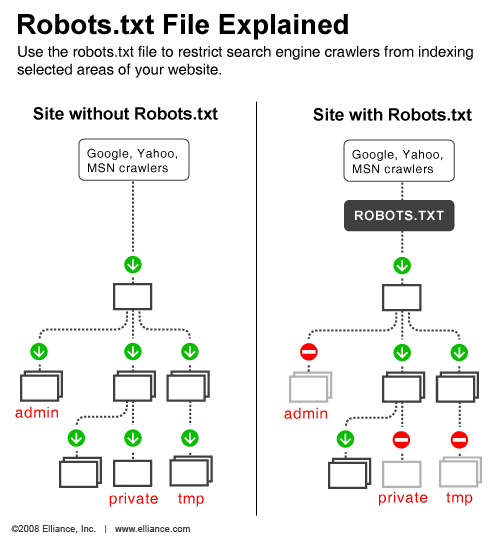
\includegraphics[width=10cm]{robot.jpg}
    \caption{Robots Exclusion Protocol }
    \label{fig-sample}
\end{figure} 
\end{itemize} 
\end{enumerate}
\subsection{Industrial analyse}
After WRSC, occasionally discussed with some Finnish engineers, we found out that they had developed a similar tracking product in order to follow the trace(\url{http://www.thingsee.com/}) based on language c  and Microsoft .net. Comparing to our tracking system, they had much more sensors, so they can measure more parameters, like: temperature, motion, orientation and so on, and their own OS based on Nuttx, the official declaration of lifetime is more than 1 year. The price of their product is more than 300 Euros. Although our tracking system do not have the same sensors, but actually the whole price we need to pay is about all the materials including one battery, two antennae(one for GPS, one for GSM), one electronic card with SIMCOM module, a SIM card and a SD card(in case of losing internet, it is optional). The total price is less than 100 Euros.

In addition, we found another similar project from the internet, in Brittany, France.(\url{https://www.gwenneg.bzh/fr/tifiz}) With a glance of these projects, it was not impossible to develop our own product with a lower cost, more functionalities, cross platform and stable performance in the near future.
\subsection{Personal analyse}
\begin{itemize}
\item{\textbf{Technical benefits}}

Thanks to this opportunity, I am able to master the development by using the ruby on rails framework, also with the front end design technologies(CSS, HTML, JavaScript). In addition, I am capable to cooperate with other developers not only with my workmates, but also include many other open source projects' developers. Keep a readable and clear coding habit, sum up the functionalities, provide well-explained APIs with concrete examples, would save a lot of time for the following developer and speed up the whole development, to make it become the real agile development.

\item{\textbf{Professional career}}

It is a good experience to work with so many kind and smart people in such a beautiful place. The internship reached my expectation, not only it meets the technical requirements, but also it satisfies my personal self-feelings.The project of Tracking system is quite a good example to discover the method of technical development. This project started from 2013, and it is enhanced year by year by different developers. It covers and shows different developments in multi-domains. A RESTful web site, an Android application and reasonable electronic cards, and all these different services share the same usable APIs. It is a good example to define our own protocol. We are individuals, but we are not alone, the well-defined protocol make it possible to communicate with the previous developers and restart from their fruit, even the different developers may stay in different eras. Further the model driven development and test driven development focus on the global view, it is a systematic and efficient way to develop any other system.

\end{itemize}
